% R08 manuscript fragment. Requires amsmath, amssymb and graphicx.
% Exact evidence and trust boundary: PROOF.md and results/*.json.
% Not compiled as a standalone document; no priority claim is made here.
\section{Exact cusp pinning and finite fold transport}

Let
\[
 F(t;\lambda,\mu,\nu)=\int_0^\infty\Phi(u)
 e^{\lambda u^2+\mu u^4+\nu u^6}\cos(2tu)\,du
\]
with the theta kernel fixed throughout the paper. Denote by
$Q=(t_Q,\lambda_Q,\mu_Q)$ the previously certified exact quartic cusp,
with $\nu=0$. All occurrences of $Q$ below refer to this exact root,
not to rounded numerical coordinates.

For $0\leq n\leq2$ and $1\leq j\leq4$, define
\[
 A_{nj}=\left.\partial_t^n\int_0^\infty\Phi(u)
 e^{\lambda_Q u^2+\mu_Q u^4}\cos(2ju)\cos(2tu)\,du
 \right|_{t=t_Q}.
\]
Set $a_j=(-1)^{j-1}\det A_{\widehat j}$,
$Z=\sum_j|a_j|$, $w_j=a_j/Z$, and
$h_0(u)=\sum_{j=1}^4w_j\cos(2ju)$.
The certified cofactors give $Z>0$ and $\|h_0\|_\infty=1$.
Let $H$ denote the integral defining $F$ with the additional factor
$h_0$, and put $F_\epsilon=F+\epsilon H$.
The cofactor identity gives $H(Q)=H_t(Q)=H_{tt}(Q)=0$ exactly.

\paragraph{Computer-assisted theorem.}
For every $(\nu,\epsilon)\in[-29,0]\times[-1/2,1/2]$, the specified
uniqueness tubes contain a single real analytic cusp graph
$c(\nu,\epsilon)=(t_*,\lambda_*,\mu_*)$ satisfying
\[
 F_\epsilon=(F_\epsilon)_t=(F_\epsilon)_{tt}=0,\qquad
 (F_\epsilon)_{ttt}>0>(F_\epsilon)_{tttt},\qquad
 0.26<\partial_\nu\mu_*<0.34.
\]
Its edge $c(0,\epsilon)$ equals $Q$ exactly. For each $\epsilon$,
the graph crosses $\mu_*=0$ exactly once on the certified driver
interval. The kernels $\Phi(1+\epsilon h_0)$ remain positive.

Use the translated, unrescaled coordinates
$s=t-t_*$, $\ell=\lambda-\lambda_*$ and $m=\mu-\mu_*$.
In the common window
\[
 |s|\leq0.003,\qquad |\ell|\leq10^{-6},\qquad |m|\leq2\,10^{-9},
\]
the discriminant consists of the cusp and two fold branches
$m_-(\ell,\nu,\epsilon)<0<m_+(\ell,\nu,\epsilon)$ for
$0<\ell\leq10^{-6}$. Between the folds there are exactly three
simple real zeros in the stated $s$ window; off the discriminant
outside this strip there is exactly one. At a noncusp fold there
are one double and one simple zero; at the cusp there is one
triple zero. No zero crosses the $s$-window boundary.

For $W=m_+-m_-$ and throughout this positive-$\ell$ window,
\[
 \partial_\nu m_+<0<\partial_\nu m_-,
 \qquad
 \partial_\epsilon m_+<0<\partial_\epsilon m_-,
\]
\[
 0.0003\,\ell^{3/2}<-\partial_\nu W<0.003\,\ell^{3/2},
 \qquad
 0.0002\,\ell^{3/2}<-\partial_\epsilon W<0.005\,\ell^{3/2}.
\]
Thus the centered three-root strips strictly widen as $\nu$
decreases and strictly narrow as $\epsilon$ increases.
No inclusion in fixed absolute $(\lambda,\mu)$ coordinates is asserted.

\paragraph{Normalization and continuation.}
Put $\alpha=H_{ttt}(Q)/F_{ttt}(Q)$,
$K=H-\alpha F$, $\rho=\epsilon/(1+\alpha\epsilon)$ and
$G=F+\rho K$. Then
$F_\epsilon=(1+\alpha\epsilon)G$, with positive prefactor.
The physical amplitudes map into $[-1/2,3/4]$ in $\rho$.
Four adjacent $\rho$ slabs and 58 $\nu$ intervals give 232
parameter cells. The uniform contraction inequalities satisfy
$q+\eta<0.258$. There are 228 root-containment joins in the
$\nu$ direction and 174 common-uniqueness-box joins in the
$\rho$ direction. These joins establish a single analytic
graph and identify its fixed $Q$ edge.

\paragraph{Transport for a general driver.}
For $\sigma=\nu$ or $\rho$, let $R=G_\sigma$ and
$G_n=\partial_t^nG$, $R_n=\partial_t^nR$. The heat identities
$\partial_\lambda G_n=-G_{n+2}/4$ and
$\partial_\mu G_n=G_{n+4}/16$, and their counterparts for $R$,
give at the cusp
\[
 \mu_\sigma=-16R_0/G_4,\qquad
 \lambda_\sigma=(4R_1+G_5\mu_\sigma/4)/G_3.
\]
On an implicit fold, differentiation at fixed relative $\ell$ yields
\[
 \partial_\sigma m=B_\sigma(s)-\mu_\sigma,\qquad
 B_\sigma(s)=\frac{4\lambda_\sigma G_2-16R_0}{G_4}.
\]
Writing $k=-G_3/G_4$ and
$A_3=\frac43(G_5/G_4-G_4/G_3)$ at the cusp, the local fold
expansion is
\[
 \ell(s)=2s^2+A_3s^3+O(s^4),\qquad
 m(s)=-\frac{16}{3}ks^3-4s^4+O(s^5).
\]
Consequently
\[
 B_\sigma(0)=\mu_\sigma,\quad
 B_\sigma'(0)=B_\sigma''(0)=0,\quad
 B_\sigma'''(0)=-32k_\sigma,\quad
 B_\sigma''''(0)=96k(A_3)_\sigma .
\]
For $\sigma=\nu$, use $R_n=-G_{n+6}/64$; for $\sigma=\rho$,
use $R_n=K_n$. Correlated Taylor models give $k_\nu,k_\rho<0$,
and explicit fourth- and fifth-derivative bounds establish
$B_\sigma'''(s)>0$ for $|s|\leq3/4000$.
The negative-$s$ fold is the upper branch, proving both nesting
directions. The quadratic bound
$\ell(s)>1.80s^2$ ensures that this interval covers every
$0<\ell\leq10^{-6}$. Finally
$\rho_\epsilon=(1+\alpha\epsilon)^{-2}>0$ gives the stated
physical-amplitude bounds.

\paragraph{Finite quantitative comparison.}
At $\ell=10^{-6}$ the certified percentage changes
$100[W(\nu,+1/2)/W(\nu,-1/2)-1]$ lie in
\[
\begin{array}{c|c}
 \nu & \text{finite width change, percent}\\ \hline
 0 & [-0.05201561,-0.05201560]\\
 -15 & [-0.04707662,-0.04707661]\\
 -29 & [-0.04254131,-0.04254130]
\end{array}
\]
These are finite-fold calculations, not evaluations of the
leading coefficient in $W=C\ell^{3/2}+O(\ell^2)$.
In particular, at $Q$ the exact position remains fixed while
\[
 C(0,\epsilon)=C(0,0)
 \frac{1+\alpha\epsilon}{1+\gamma\epsilon},
 \qquad
 \gamma=H_{tttt}(Q)/F_{tttt}(Q),
\]
varies with $\epsilon$.

\paragraph{Verification scope.}
The package includes 4002 new rigorously bounded central $H$ moments,
the full two-parameter contraction certificate, a separate rational
check of all continuation and geometry inequalities, and an
independent fold-ODE reconstruction of the fifth transport derivatives.
The rational check assumes the saved integral and correlated
two-variable Taylor enclosures; it does not independently regenerate
that entire upstream stage. Selected integral comparisons and
separate rational checks of 21 cusp and 144 fold samples supplement
the continuum argument. The theorem concerns only the chosen
cofactor direction and stated local windows; no global zero count,
optimal amplitude, or physical stability claim follows.

% Suggested figure inclusions, relative to this fragment's directory:
% 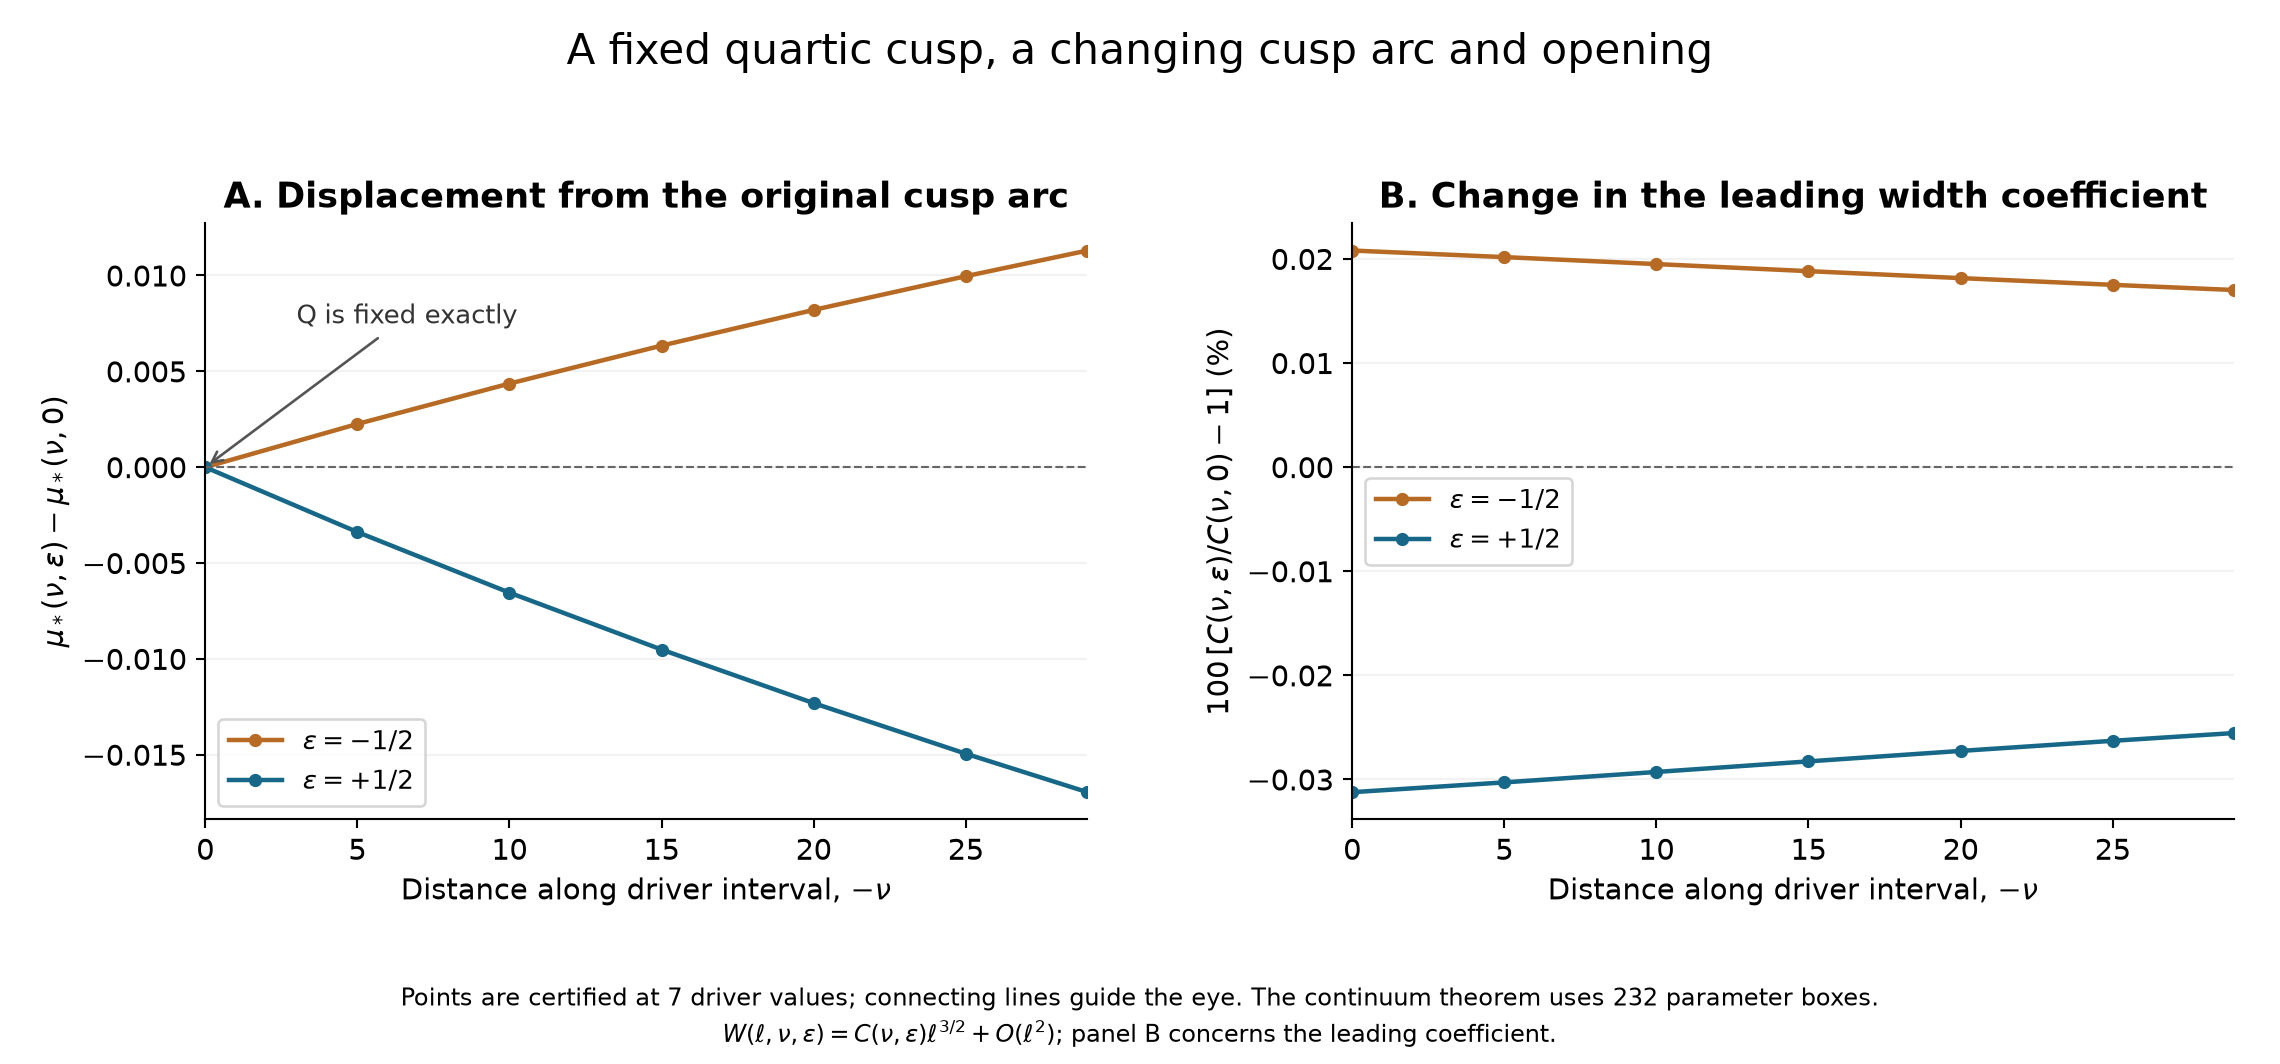
\includegraphics[width=\textwidth]{figures/pinned_cusp_sheet.png}
% 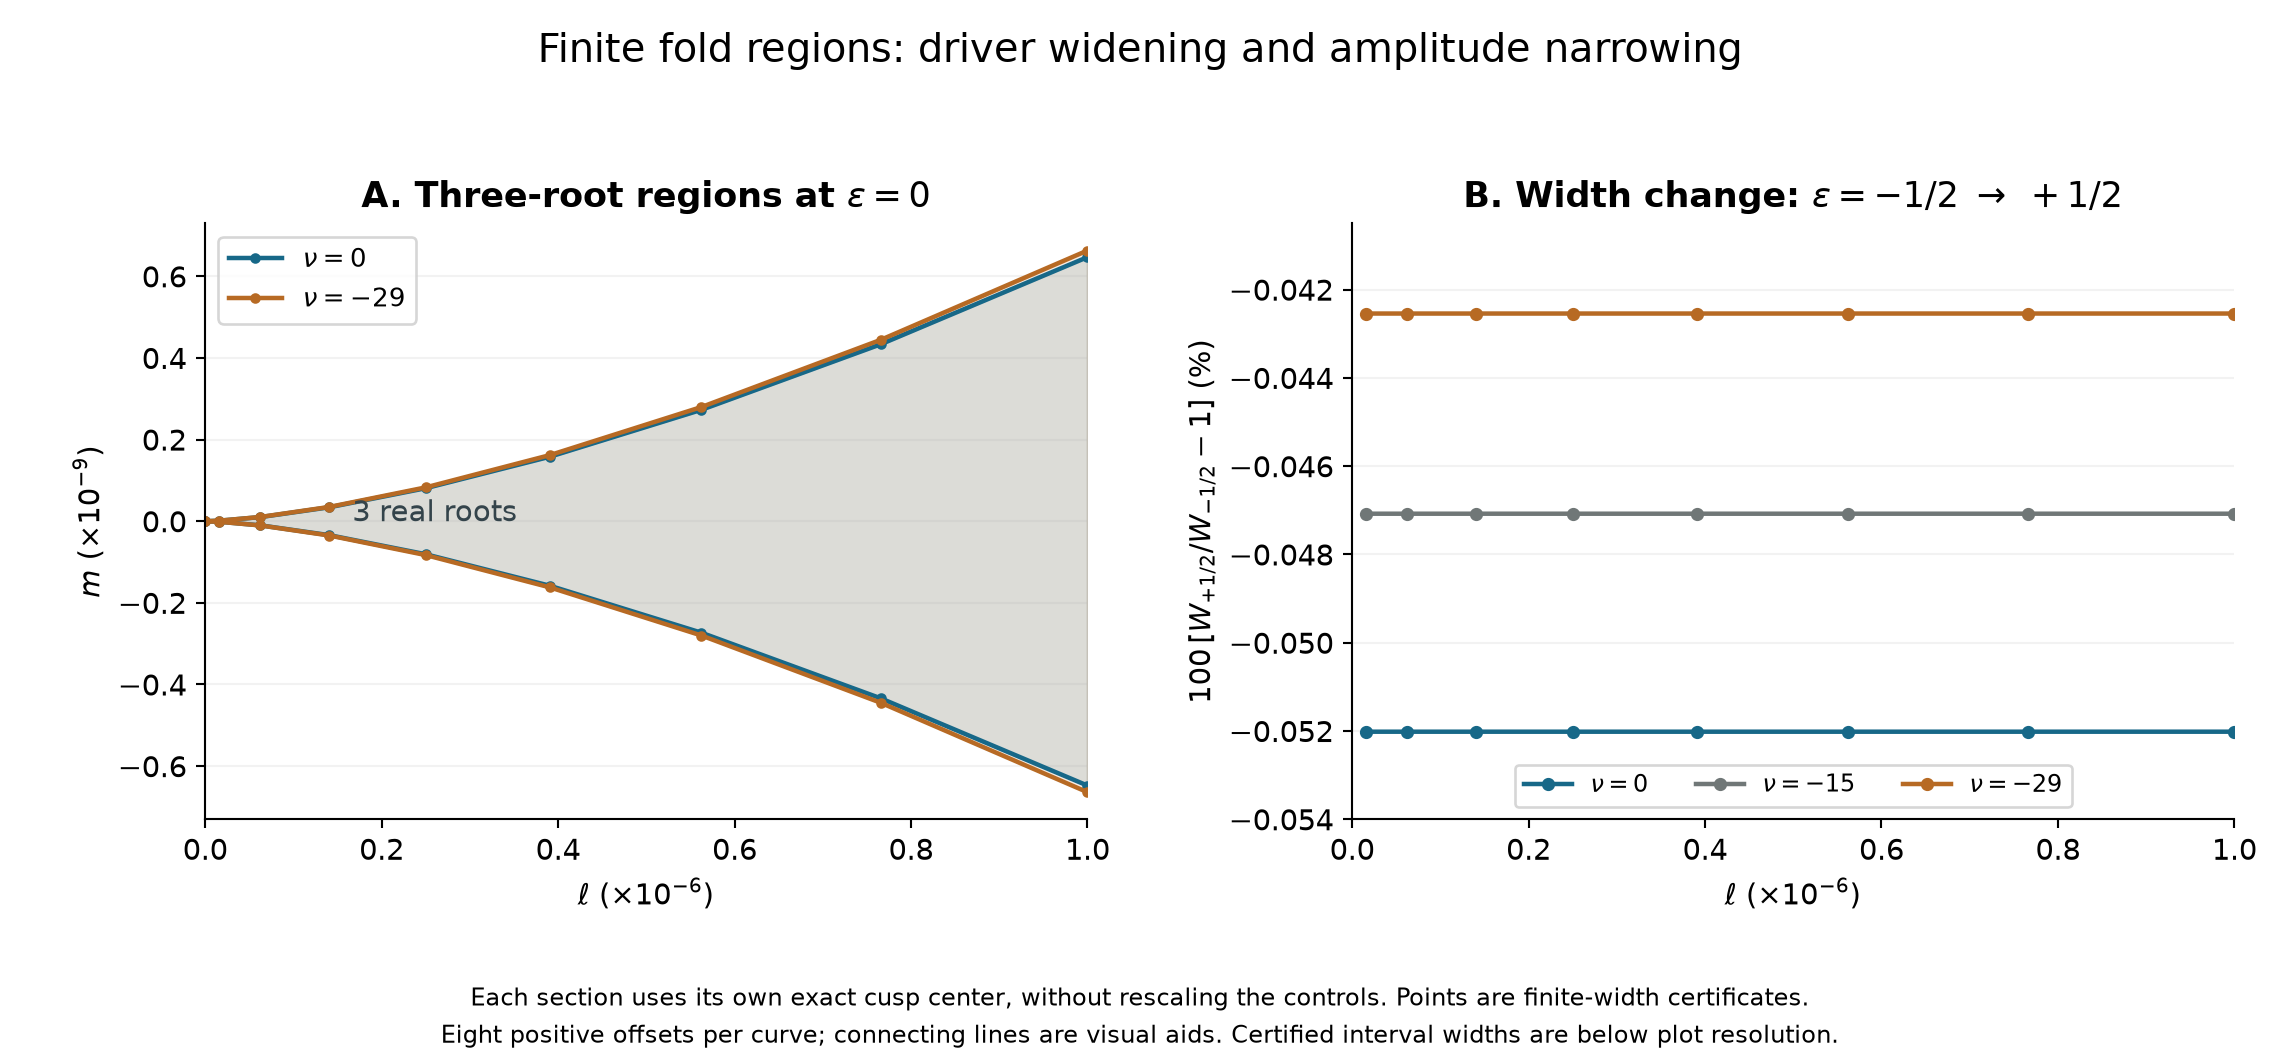
\includegraphics[width=\textwidth]{figures/finite_fold_comparison.png}
% Connecting lines are visual aids; only the displayed points and the
% separately certified continuum inequalities enter the evidence.
